% The LaTeX cookbook: every slide pattern a LaTeX author can use, the twin of the Quarto
% cookbook decks/sample/sample.qmd, slide for slide (latex/authoring.md walks through it).
%
% Build (here):   make examples        -> examples/sample.pdf
% Variants:       make variants        -> sample-nasa-dark.pdf (a dark livery), sample-cu.pdf, sample-43.pdf
% Contact sheet:  make previews        -> ../sample.png (the pattern slides under three liveries)
%
\providecommand\enginethemeoptions{}      % the variants' hook: livery=..., fonts=bundled, ...
\providecommand\engineaspectratio{169}
\documentclass[aspectratio=\engineaspectratio]{beamer}

\usepackage{booktabs}
\usepackage{listings}
\usepackage{varwidth}     % a list centered as a block (the "filled" slide)
% citations: biblatex, author-year, run by bibtex (latexmk runs it); biber: backend=biber
\usepackage[style=authoryear,backend=bibtex]{biblatex}
\addbibresource{references.bib}

% livery=liveries/<name>|<dir>   title=dark|light   footer=minimal|full   mathfont=serif|stix|sans|...
% typescale=0.9 sizes every slide's text
\usetheme[livery=liveries/ncar,\enginethemeoptions]{Engine}
% \enginemarking{CUI}   % the livery's first marking strip on every slide ([<name>] another; {} for none)

\title{LaTeX for HPC Documentation}
\subtitle{A Cookbook of Slide Patterns}
\author{Your Name, NCAR/CISL}
\institute{Computational \& Information Systems Laboratory}
\date{\today}
% \titlegraphic{\includegraphics{photo.jpg}}   % over the livery's default photo; \enginenotitlegraphic for none

\begin{document}

\begin{frame}[plain,noframenumbering]
  \titlepage
\end{frame}

\begin{frame}{Agenda}
  % the numbered sections, from \section's table-of-contents lines (a second run: latexmk's), each
  % \sectionsubtitle under its title; placed in a section, that one is current (see Wrap-up)
  \engineagenda
\end{frame}

%%%%%%%%%%%%%%%%%%%%%%%%%%%%%%%%%%%%%%%%%%%%%%%%%%%%%%%%%%%%%%%%%%%%%%%%%%%%%%
\sectionsubtitle{A \texttt{\textbackslash sectionsubtitle} before the section is the divider's subtitle.}
\section{Basics}

\begin{frame}{Text \& inline formatting}
  Plain prose with \textbf{bold}, \emph{italic}, and \texttt{inline code}. Hyperlinks look
  like \href{https://www.latex-project.org/}{the LaTeX project}. \alert{Alerted text} is
  emphasized in the brand's alert color.

  Bulleted list:
  \begin{itemize}
  \item First point
  \item Second point with \texttt{code}. This point needs to be expounded upon very very
    verbosely to force a line wrap so we can see how spacing works for wrapped bullets.
    \begin{itemize}
    \item Especially when there are multiple. And one also needs to be expounded upon very
      very verbosely to force a line wrap so we can see how spacing works for wrapped sub-bullets.
    \item Sub-bullets
    \end{itemize}
  \item Third point
  \end{itemize}

  Numbered list:
  \begin{enumerate}
  \item Step one
  \item Step two
  \item Step three
  \end{enumerate}
\end{frame}

\begin{frame}{Wall of Text.}
  % \small steps the body down one size; \begin{enginescale}{0.85} ... \end{enginescale} scales
  % the body, its tables and code by a factor (the "warning" and "short table" slides below)
  \small
  We use this slide to see how wrapping works with a lot of text.

  \emph{Lorem ipsum dolor sit amet consectetur adipiscing elit. Quisque faucibus ex sapien vitae
  pellentesque sem placerat. In id cursus mi pretium tellus duis convallis. Tempus leo eu aenean
  sed diam urna tempor. Pulvinar vivamus fringilla lacus nec metus bibendum egestas. Iaculis massa
  nisl malesuada lacinia integer nunc posuere. Ut hendrerit semper vel class aptent taciti
  sociosqu. Ad litora torquent per conubia nostra inceptos himenaeos.}

  \emph{Lorem ipsum dolor sit amet consectetur adipiscing elit. Quisque faucibus ex sapien vitae
  pellentesque sem placerat. In id cursus mi pretium tellus duis convallis. Tempus leo eu aenean
  sed diam urna tempor. Pulvinar vivamus fringilla lacus nec metus bibendum egestas. Iaculis massa
  nisl malesuada lacinia integer nunc posuere. Ut hendrerit semper vel class aptent taciti
  sociosqu. Ad litora torquent per conubia nostra inceptos himenaeos.}
\end{frame}

\begin{frame}{Math}
  Inline math reads like $E = mc^2$ inside a sentence.

  Display math gets its own line. Amdahl's law:
  \begin{equation*}
    S(p) \;=\; \frac{1}{(1 - f) + f / p}
  \end{equation*}
  where $f$ is the parallel fraction and $p$ is the processor count. The theme sets math in a
  serif math font beside the brand's sans; \texttt{\textbackslash usetheme[mathfont=stix]\{Engine\}}
  (or \texttt{lm}, \texttt{pagella}, \texttt{sans}, \texttt{poppins}) picks another.
\end{frame}

\begin{frame}{A pull quote}
  \begin{enginequote}{Richard Hamming, 1962}   % [role=accent] colors the bar; {} for no attribution
    The purpose of computing is insight, not numbers.
  \end{enginequote}
  An \texttt{enginequote} sets its lines in the quote size beside a bar (\texttt{role=} picks its
  color), the attribution under them.
\end{frame}

\begin{frame}{Tables}
  % a hand-written tabular is left alone; these draw it as the theme draws a Quarto table:
  % \engineth for a header cell, the brand rule under the header, a light rule at the foot,
  % \rowcolor{enginetableband} on every second row (\arrayrulecolor is global: set it per table)
  \centering
  \begin{tabular}{lcr}
    \engineth{Resource} & \engineth{Type} & \engineth{Cores per node} \\
    \arrayrulecolor{BrandPrimaryContrast}\specialrule{1.5pt}{0.3ex}{0pt}
    Derecho & HPC & 128 \\
    \rowcolor{enginetableband} Casper & DAV & 36 \\
    Gust & HPC & 128 \\
    \arrayrulecolor{enginetablerule}\specialrule{0.6pt}{0pt}{0pt}
  \end{tabular}
  \enginenote{Sample HPC resources}
  \note{Column alignment is the tabular's preamble: l, c, r.}
\end{frame}

\begin{frame}{Citing sources}
  % biblatex's commands: \parencite (Author Year), \textcite (Author (Year)), \footcite (a
  % footnote at the frame's foot, in the theme's look); the list is \printbibliography
  MPAS solves the compressible equations on a C-grid \parencite{skamarock2012}; see also
  \textcite{knuth84}.
  \medskip

  A footnote citation\footcite{quarto} is beamer's own footnote, set at the foot of the frame
  under the theme's short rule, its mark in the accent.
\end{frame}

%%%%%%%%%%%%%%%%%%%%%%%%%%%%%%%%%%%%%%%%%%%%%%%%%%%%%%%%%%%%%%%%%%%%%%%%%%%%%%
\section{Layouts}

\begin{frame}[fragile]{Two-column layout}
  % enginecolumns{<weights>}: each column its share of the text width less the livery's gap
  \begin{enginecolumns}{55,45}
    \enginecolumn
    \textbf{Left column --- bullets:}
    \begin{itemize}
    \item Mix any block content
    \item Bullets, prose, tables
    \item Adjust width per side
    \end{itemize}
    \enginecolumn
    \textbf{Right column --- code:}
\begin{lstlisting}[language=bash]
mpirun -n 4 ./a.out
\end{lstlisting}
  \end{enginecolumns}
\end{frame}

\begin{frame}{Two-thirds and one-third}
  \begin{enginecolumns}{2,1}
    \enginecolumn
    \begin{itemize}
    \item \texttt{enginecolumns\{2,1\}}: weights, or shares of the row when they add to 1 or less
    \item The gap between columns is the livery's (\texttt{boxes.columns.gap})
    \item \texttt{\textbackslash enginecolumn} starts each column; the livery's rule between them,
      when it draws one
    \end{itemize}
    \enginecolumn
    \includegraphics[width=\linewidth]{images/wallpaper/mesa_lab.jpg}
  \end{enginecolumns}
\end{frame}

\begin{frame}{Three plain columns}
  \begin{enginecolumns}{3}
    \enginecolumn
    \textbf{Compute}
    \begin{itemize}
    \item CPU nodes
    \item GPU nodes
    \end{itemize}
    \enginecolumn
    \textbf{Storage}
    \begin{itemize}
    \item Scratch
    \item Campaign
    \end{itemize}
    \enginecolumn
    \textbf{Analysis}
    \begin{itemize}
    \item JupyterHub
    \item Visualization
    \end{itemize}
  \end{enginecolumns}
\end{frame}

\begin{frame}{Four columns on a wide slide}
  % enginewide: the body widens to the slide less geometry.wide-margin a side
  \begin{enginewide}
    \begin{enginecolumns}{4}
      \enginecolumn
      \textbf{Plan.} \texttt{enginewide} round the body widens it to the slide less a narrower margin.
      \enginecolumn
      \textbf{Build.} Room for three or four columns, or a wide table.
      \enginecolumn
      \textbf{Run.} A livery that sets a column rule draws it in each gap.
      \enginecolumn
      \textbf{Check.} Look at the PDF: beamer has no autofit.
    \end{enginecolumns}
  \end{enginewide}
\end{frame}

\begin{frame}{Options side by side}
  % enginelead: a lead box over the row; enginecards{3}: three equal cards (or weights, {2,1,1});
  % enginecard[<keys>]{Title}{Sub}: role= (default by place: primary, secondary, accent), pick,
  % solid, plain; {} for no sub-line. \enginelabel and \enginebig; enginestrip[role=] a band;
  % enginestatus a list of \done \warn \fail items (and plain \item)
  \begin{enginelead}
    \textbf{Three ways to spend the next allocation}\par
    Local capacity against a consortium share.
  \end{enginelead}
  \begin{enginecards}{3}
    \begin{enginecard}[pick]{OPTION 1}{A modern GPU system}
      \textbf{Total cost \$30M}
      \enginelabel{Local investment}
      \enginebig{\$20M}
      \begin{enginestrip}[role=accent]
        → \textbf{\$10M} shared out
      \end{enginestrip}
      \begin{enginestatus}
        \done Archive expansion
        \warn High-res runs
      \end{enginestatus}
    \end{enginecard}
    \begin{enginecard}{OPTION 2}{Join the consortium}
      \textbf{Total cost \$15M}
      \enginelabel{Local investment}
      \enginebig{\$5M}
      \begin{enginestatus}
        \done Shared capacity
        \fail Local control
      \end{enginestatus}
    \end{enginecard}
    \begin{enginecard}{OPTION 3}{A hybrid of both}
      \textbf{Total cost \$25M}
      \enginelabel{Local investment}
      \enginebig{\$15M}
      \begin{enginestatus}
        \warn Two systems to run
      \end{enginestatus}
    \end{enginecard}
  \end{enginecards}
\end{frame}

\begin{frame}{Options, the pick moving across steps}
  % pick=<overlay>: the outline on those steps only; its width is reserved on every step, so the
  % cards do not move. A status item takes an overlay spec too: \warn<2-> appears at step 2.
  \begin{enginecards}{3}
    \begin{enginecard}[pick=<1>]{OPTION 1}{A modern GPU system}
      \enginelabel{Local investment}
      \enginebig{\$20M}
      \begin{enginestatus}
        \done Data archive expansion
        \warn<2-> High-resolution runs
      \end{enginestatus}
    \end{enginecard}
    \begin{enginecard}[pick=<2>]{OPTION 2}{Join the consortium}
      \enginelabel{Local investment}
      \enginebig{\$5M}
      \begin{enginestatus}
        \done Shared capacity
        \fail<3-> Local control
      \end{enginestatus}
    \end{enginecard}
    \begin{enginecard}[pick=<3>]{OPTION 3}{A hybrid of both}
      \enginelabel{Local investment}
      \enginebig{\$15M}
      \begin{enginestatus}
        \warn Two systems to run
      \end{enginestatus}
    \end{enginecard}
  \end{enginecards}
\end{frame}

\begin{frame}{Solid cards}
  \begin{enginecards}{3}
    \begin{enginecard}[solid]{Plan}{}
      Write the slides in LaTeX, one file.
    \end{enginecard}
    \begin{enginecard}[solid]{Build}{}
      \texttt{latexmk -xelatex} renders the PDF from it.
    \end{enginecard}
    \begin{enginecard}[solid]{Share}{}
      Hand out the PDF; the same file builds on Overleaf.
    \end{enginecard}
  \end{enginecards}
\end{frame}

\begin{frame}{Steps inside cards}
  % a card's body is boxed before the row is drawn, and beamer's overlays survive that: \item<+->,
  % \pause and \uncover all work inside a card. \uncover keeps the row one height across the
  % steps; \only would make it jump.
  \begin{enginecards}{3}
    \begin{enginecard}{Item steps}{\texttt{\textbackslash item<+->}}
      \begin{itemize}
      \item<+-> First
      \item<+-> Second
      \item<+-> Third
      \end{itemize}
    \end{enginecard}
    \begin{enginecard}{Pause}{\texttt{\textbackslash pause}}
      Before the pause.

      \pause
      After the pause.
    \end{enginecard}
    \begin{enginecard}{Uncover}{\texttt{\textbackslash uncover<2->}}
      The strip appears at step 2.
      \uncover<2->{\begin{enginestrip}
        The row keeps one height
      \end{enginestrip}}
    \end{enginecard}
  \end{enginecards}
\end{frame}

\begin{frame}{A process, step by step}
  % enginesteps{n}: n equal steps on a rail, a numbered badge each in role= (default
  % primary-contrast, the primary that reads on the background);
  % each step's text is boxed before the row is drawn, as a card's, so overlays work inside it
  \begin{enginesteps}{3}
    \begin{enginestep}{Propose}
      A one-page case; the review board reads it in a week.
    \end{enginestep}
    \begin{enginestep}{Pilot}
      Six weeks on the shared system.

      \uncover<2->{A second line, at step 2.}
    \end{enginestep}
    \begin{enginestep}{Scale}
      The allocation follows the pilot's numbers.
    \end{enginestep}
  \end{enginesteps}
\end{frame}

\begin{frame}{A timeline}
  % enginetimeline{n}: n milestones on a rail, the date above each dot and the label below;
  % [done] fills the dot in role=, a milestone without it is hollow
  \begin{enginetimeline}{4}
    \enginemilestone[done]{Q1 2025}{Proposal accepted}
    \enginemilestone[done]{Q3 2025}{Pilot complete}
    \enginemilestone{2026}{Full allocation}
    \enginemilestone{2027}{First review}
  \end{enginetimeline}
\end{frame}

\begin{frame}{Six views from orbit and beyond}
  % enginegallery: \engineimage[caption]{file} per picture, in equal cells; cols= and rows= (by
  % default as square as the count allows), fit=contain (whole, the default) or cover (cropped to
  % fill), height= a share of the body box: give it under text, which TeX cannot measure
  A line above a gallery takes its own height; here \texttt{height=0.75} leaves it room.
  \begin{enginegallery}[cols=3,rows=2,height=0.75]
    \engineimage[The Blue Marble]{images/gallery-1.jpg}
    \engineimage[Earthrise]{images/gallery-2.jpg}
    \engineimage[Artemis I]{images/gallery-3.jpg}
    \engineimage[Aurora]{images/gallery-4.jpg}
    \engineimage[Helene]{images/gallery-5.jpg}
    \engineimage[Liftoff]{images/gallery-6.jpg}
  \end{enginegallery}
\end{frame}

\begin{frame}{A strip of six}
  % in enginewide, the wider body; fit=cover crops each picture to its cell
  \begin{enginewide}
  \begin{enginegallery}[cols=6,rows=1,fit=cover]
    \engineimage{images/gallery-1.jpg}\engineimage{images/gallery-2.jpg}\engineimage{images/gallery-3.jpg}
    \engineimage{images/gallery-4.jpg}\engineimage{images/gallery-5.jpg}\engineimage{images/gallery-6.jpg}
  \end{enginegallery}
  \end{enginewide}
\end{frame}

\begin{frame}[enginefull]
  % the bare enginefull key: a full frame with no picture of its own; the gallery in it fills
  % the slide less its pads, and \enginefullcaption is its caption line
  \enginefullcaption{With \texttt{[enginefull]} the cells fill the slide, and this line is the caption.}
  \begin{enginegallery}[cols=3,rows=2,fit=cover]
    \engineimage{images/gallery-1.jpg}\engineimage{images/gallery-2.jpg}\engineimage{images/gallery-3.jpg}
    \engineimage{images/gallery-4.jpg}\engineimage{images/gallery-5.jpg}\engineimage{images/gallery-6.jpg}
  \end{enginegallery}
\end{frame}

\begin{frame}{Status items, step by step}
  % enginestatus on its own: ✓ ⚠ ✗ as the bullets, in the livery's status colors; a failed
  % item's text muted. \engineglyph{done|warn|fail} is the glyph anywhere (a table cell).
  \begin{enginestatus}
    \done<1-> Image builds on both architectures
    \warn<2-> Apptainer needs the release .deb on arm64
    \fail<3-> No Keynote on any CI runner
    \item<4-> An ordinary bullet, with a glyph in the text: \engineglyph{done}
  \end{enginestatus}
\end{frame}

\begin{frame}{Image embed}
  \centering
  \includegraphics[width=0.6\linewidth]{images/wallpaper/mesa_lab.jpg}
  % \enginenote: a remark under a figure or table, in the caption's look
  \enginenote{A caption for the figure. Size it with \texttt{width=} or \texttt{height=};
    PDF, PNG and JPG all work.}
\end{frame}

\begin{frame}{A linked screenshot}
  % the picture is the link; the URL on a foot line, as a slide footnote
  \enginefootnotespring
  \centering
  \href{https://ncar.ucar.edu/}{\includegraphics[height=0.72\textheight]{images/wallpaper/mesa_lab.jpg}}
  \enginefootnotespring
  \begin{enginefootnotes}
    \enginefootnote{†}{\url{https://ncar.ucar.edu/}}
  \end{enginefootnotes}
\end{frame}

\begin{frame}[enginebg=images/wallpaper/mesa_lab.jpg]{Full-bleed photo}
  \begin{enginefeaturepanel}
    \texttt{[enginebg=<photo>]} makes a full-bleed photo slide, in the livery's
    \texttt{feature.style}: the title on a dark bar and the text on a translucent panel
    (\texttt{bar}), or the title cover's field and waves with the photo beside them
    (\texttt{cover}).
  \end{enginefeaturepanel}
\end{frame}

% [enginefull=<image>]: the whole picture, uncropped; no title, logo or rule is drawn
\begin{frame}[enginefull=images/wallpaper/mesa_lab.jpg]
  \enginefullcaption{\texttt{[enginefull=<image>]}: the whole picture, uncropped;
    \texttt{enginebg} crops a photo to cover.}
  \note{A full frame takes one image, then an optional \texttt{\textbackslash enginefullcaption}.}
\end{frame}

\begin{frame}{A list, step by step}
  % beamer's overlays: <+-> reveals the items one at a time (one page per step)
  \begin{itemize}
  \item<+-> \texttt{\textbackslash item<+->} reveals a list one item at a time
  \item<+-> one PDF page per step
  \item<+-> a dark slide is the dark livery's: \texttt{make variants} builds this deck under
    \texttt{nasa-dark}
  \end{itemize}
\end{frame}

\begin{frame}[c]{⚠︎ A warning slide}
  % [c] centers the body; enginescale{1.15} sizes it; enginecaution sets it on the soft yellow
  % field with the brand-yellow bar; the footnote stays below the box
  \enginefootnotespring
  \begin{enginescale}{1.15}
    \begin{enginecaution}
      \begin{itemize}
      \item \texttt{enginecaution} sets the body on a soft yellow field, with a brand-yellow bar.
      \item Keep it for the slides that warn: the brand asks for accents in small amounts.
      \item It combines with the other layout controls, here \texttt{[c]} and \texttt{enginescale}.
      \end{itemize}
    \end{enginecaution}
  \end{enginescale}
  \enginefootnotespring
  \begin{enginefootnotes}
    \enginefootnote{†}{\emph{Footnotes stay below the box.}}
  \end{enginefootnotes}
\end{frame}

\begin{frame}[c]{A short table, centered and scaled}
  \begin{enginescale}{1.4}
    \centering
    \begin{tabular}{ll}
      \engineth{Control} & \engineth{Moves} \\
      \arrayrulecolor{BrandPrimaryContrast}\specialrule{1.5pt}{0.3ex}{0pt}
      \texttt{[c]} & the body, down \\
      \rowcolor{enginetableband} \texttt{\textbackslash centering} & the body, across \\
      \texttt{enginescale\{S\}} & its size \\
      \rowcolor{enginetableband} \texttt{[shrink]} & down to fit (beamer's own) \\
      \arrayrulecolor{enginetablerule}\specialrule{0.6pt}{0pt}{0pt}
    \end{tabular}
  \end{enginescale}
  \note{Each control is independent; the title, these notes and any footnote are left alone.}
\end{frame}

\begin{frame}{A short list, filled}
  % enginescale grows the body; center + varwidth centers a list as a block
  \begin{enginescale}{1.3}
    \begin{center}\begin{varwidth}{\linewidth}
      \begin{itemize}
      \item \texttt{enginescale\{1.3\}} grows the body (beamer has no autofit)
      \item \texttt{[shrink]} on the frame goes the other way: down to fit
      \item \texttt{varwidth} in \texttt{center} centers the list as a block
      \end{itemize}
    \end{varwidth}\end{center}
  \end{enginescale}
\end{frame}

%%%%%%%%%%%%%%%%%%%%%%%%%%%%%%%%%%%%%%%%%%%%%%%%%%%%%%%%%%%%%%%%%%%%%%%%%%%%%%
\section{Code \& Diagrams}

\begin{frame}[fragile]{Static code blocks}
  Bash, with syntax highlighting only (not executed):
\begin{lstlisting}[language=bash]
#!/usr/bin/env bash
module load intel openmpi
mpirun -n 8 ./solver --grid 256
\end{lstlisting}
  Python:
\begin{lstlisting}[language=Python]
import numpy as np

def speedup(f, p):
    return 1.0 / ((1 - f) + f / p)

print(speedup(0.95, 64))
\end{lstlisting}
\end{frame}

\begin{frame}[fragile]{Showing captured shell output}
  Nothing runs at build time: capture a session to a file, then
  \texttt{\textbackslash lstinputlisting} it.
  \lstinputlisting{snippets/terminal/whoami.session}
  \note{A Quarto deck runs a code cell when it renders; a LaTeX deck shows what you captured.}
\end{frame}

% diagrams/*.pdf come from the .mmd and .dot beside them (`make diagrams`): a diagram is a
% picture here, rendered once, outside the deck
\begin{frame}{Mermaid diagram}
  \enginefootnotespring
  \centering
  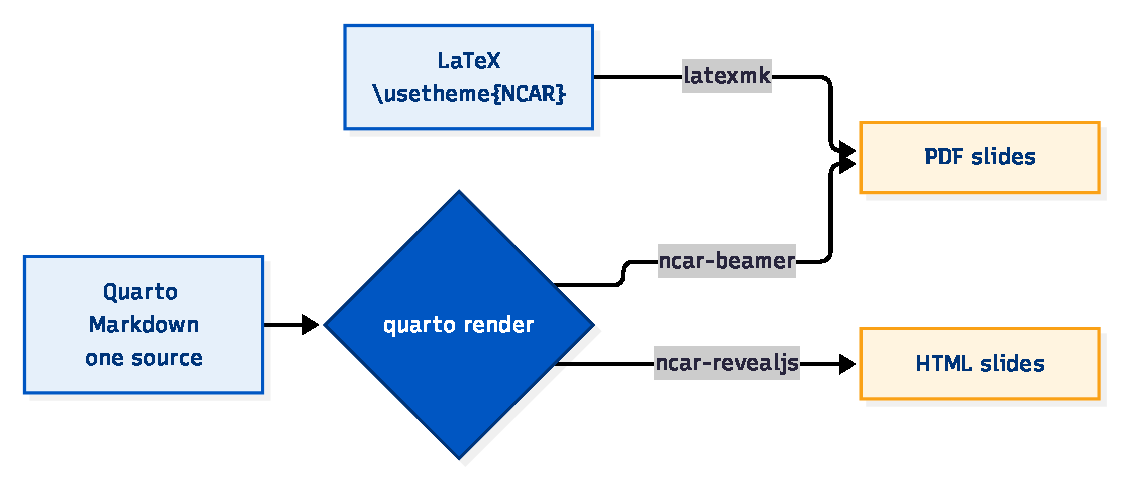
\includegraphics[width=\linewidth,height=0.6\textheight,keepaspectratio]{diagrams/render.pdf}
  \enginenote{One short label a box keeps a left-to-right flow near the slide's 2.4:1.}
  \enginefootnotespring
  \begin{enginefootnotes}
    \enginefootnote{†}{\texttt{make diagrams} renders \texttt{diagrams/render.mmd} with
      mermaid-cli; the deck includes the PDF.}
  \end{enginefootnotes}
\end{frame}

\begin{frame}{Graphviz diagram}
  \centering
  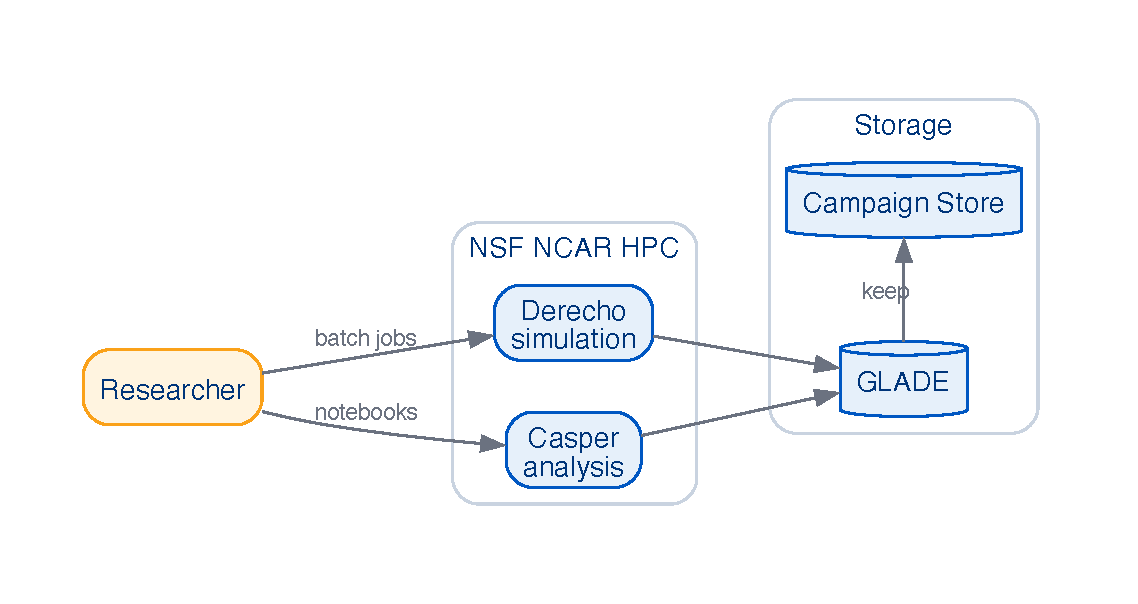
\includegraphics[width=\linewidth,height=0.7\textheight,keepaspectratio]{diagrams/systems.pdf}
  \enginenote{\texttt{dot -Tpdf} on \texttt{diagrams/systems.dot}: clusters keep their layout.}
\end{frame}

\begin{frame}{Speaker notes}
  The body of this slide is short on purpose.
  % \setbeameroption{show notes} in the preamble shows every \note on a page of its own
  % (show notes on second screen=right puts them beside the slide)
  \note{Speaker notes go in \texttt{\textbackslash note\{...\}} and are shown only under
    \texttt{\textbackslash setbeameroption\{show notes\}}. Use them for talking points,
    citations, or reminders that should not clutter the projected slide.}
\end{frame}

%%%%%%%%%%%%%%%%%%%%%%%%%%%%%%%%%%%%%%%%%%%%%%%%%%%%%%%%%%%%%%%%%%%%%%%%%%%%%%
\section{Wrap-up}

\begin{frame}{Where we are}
  \engineagenda
\end{frame}

\begin{frame}{Next steps}
  % slide footnotes: a spring first, the content, a spring, then the footnotes
  \enginefootnotespring
  \begin{itemize}
  \item Copy this file as a starting point for new decks, or start from \texttt{talk.tex}.
  \item \texttt{examples/template.tex} shows the theme's blocks, palette and fonts.
  \item Build with \texttt{latexmk -xelatex} from this directory, or on Overleaf.
  \item Drop images under \texttt{images/} and \texttt{\textbackslash includegraphics} them.
  \end{itemize}
  \enginefootnotespring
  \begin{enginefootnotes}
    \enginefootnote{†}{A slide footnote: at the foot under a short rule, the marker in the
      accent color.}
    \enginefootnote{‡}{\emph{A second one stacks under the first, in order; emphasis is kept.}}
  \end{enginefootnotes}
\end{frame}

\begin{frame}[allowframebreaks]{References}
  % allowframebreaks: a long list runs on over as many pages as it needs, (1), (2)
  \printbibliography[heading=none]
\end{frame}

\engineclosingframe{Thank you!}{%
  \texttt{\textbackslash engineclosingframe} makes a closing slide on the brand field, with this
  text under the headline.\par\medskip
  Questions: \texttt{your.name@ucar.edu}}

%%%%%%%%%%%%%%%%%%%%%%%%%%%%%%%%%%%%%%%%%%%%%%%%%%%%%%%%%%%%%%%%%%%%%%%%%%%%%%
% a divider outside the count: no eyebrow, not on the agenda (no \section, so no bookmark either)
\enginesectionunnumbered{Backup}{}

\begin{frame}[fragile]{Project config: \texttt{latexmkrc}}
  % \lstinputlisting pastes a file at build time, so the slide stays in sync with it
  \lstinputlisting[language=Perl,breaklines=true]{latexmkrc}
  \note{This is the \texttt{latexmkrc} TeX finds on its path: the one beside this deck's
    Makefile, or the one at an Overleaf project's root. It points TeX at the theme and the
    liveries; nothing else is set.}
\end{frame}

\begin{frame}{What \texttt{\textbackslash usetheme} sets}
  \begin{enginescale}{0.85}
    \begin{enginecolumns}{2}
      \enginecolumn
      \textbf{The livery}
      \begin{itemize}
      \item \texttt{livery=liveries/<name>}: the brand's colors, fonts, logos, geometry and art,
        found through \texttt{TEXINPUTS}; any directory holding \texttt{build/livery.sty} works.
      \item \texttt{fonts=bundled}: the livery's font files (what Overleaf gets); \texttt{brand}
        uses the installed faces when this machine has them.
      \item \texttt{title=light}: the brand's light cover.
      \end{itemize}
      \enginecolumn
      \textbf{The deck}
      \begin{itemize}
      \item \texttt{footer=full}: section, short title and date beside the page number.
      \item \texttt{typescale=0.9}: every text size times it.
      \item \texttt{mathfont=stix}: the math font.
      \item \texttt{waves=false}, \texttt{logo=false}, \texttt{sectionpages=false}: the
        furniture off.
      \end{itemize}
    \end{enginecolumns}
  \end{enginescale}
\end{frame}

\end{document}
